\documentclass{ctexart}
\makeatletter
\def\@cite#1#2{\textsuperscript{[{#1\if@tempswa , #2\fi}]}}
\makeatother
\usepackage{amsmath}
\usepackage{bm}
\usepackage{graphicx}
\usepackage{diagbox}
\usepackage{multirow}
%\usepackage{multicolumn}
\usepackage{amssymb}
\usepackage{geometry}
\usepackage{fancyhdr}
\usepackage{minted}
\geometry{a4paper,left=3cm,right=3cm,top=3cm,bottom=3cm}

\pagestyle{fancy}
\lhead{{\songti 吉林大学学士学位论文}}
\chead{}
\rhead{\leftmark}
\begin{document}
\thispagestyle{plain}
\pagenumbering{Roman}
\section*{摘要}

为了在降水机理不明确,气象资料不完全的情况预测月降水量,提出了基于PCA的树增型朴素贝叶斯分类器的模型。本文以美国马塞纳国际机场的数据为例,运用交叉验证法划分训练集和测试集,将主成分分析降维后的数据用于构造贝叶斯网,根据贝叶斯网和先验概率估算出降水类别。并将此模型与时间序列分析法,人工神经网络模型根据$F$-measure方法进行对比。结果表明,相比于ARIMA模型,BP神经网络模型,基于PCA的树增强型朴素贝叶斯分类器具有精确度高,计算复杂度低的优点。
\newline
\newline
\textbf{关键词:}\ 树增型朴素贝叶斯算法,\ PCA,\ ARIMA模型,\ BP神经网络
\section*{Abstract}
In order to predict monthly precipitation at the circumstance that the mechanism of precipitation is not clear and the meteorological data are incomplete, Tree Augmented Naïve Bayesian Classifier based on PCA is proposed. Taking the data of Massena International Airport as an example, the Cross Validation Method is used to divide training set and test set. The dimensionally reduced data based on Principal Component Analysis is used to construct Bayesian network, and the precipitation types are estimated according to Bayesian network and prior probability. The model is compared with the Time Series Analysis method and the Artificial Neural Network model according to the $F$-measure method. The results show that, compared with ARIMA model, BP Neural Network model, Tree Augmented Naïve Bayesian Classifier based on PCA has the advantages of high accuracy and low computational complexity.
\newline
\newline
\textbf{Keywords:}\ Tree Augmented Naïve Bayesian Model,\ Principal Component Analysis,\ ARIMA Model,\ BP Neural Network
\newpage
\thispagestyle{plain}
\setcounter{page}{1}
\tableofcontents
\newpage
\pagenumbering{arabic}
\setcounter{page}{1}
\section{绪论}
\subsection{研究背景和意义}
   人们尝试去预测天气已经有上千年的历史了。在公元前650年,巴比伦人运用云的形状和占星术去预测天气,在公元前350年,亚里士多德将天气情况写入``气候通典''中。中国的关于天气预测的传说可以追溯到公元300年前,在此同时,印度天文学家也总结出了天气预测的方法。古代天气预测方法通常依赖于可观测的事件的状态,例如,如果日落时的太阳十分红,那么下一天的天气经常会是好的。这种一代一代积累的经验变成了天气法则。然而,不是所有的这种预言都是可靠的,并且他们当中的许多观点在现代严格的统计测试中都不成立。

直到1835年电报的发明,近代天气预报才开始。电报使人们几乎可以在瞬间收到来自广袤地区的天气状况报告,使人们能够根据对天气状况的了解做出预报。20世纪初期,人们开始用电视传播天气预报。20世纪中后期,随着卫星技术和计算机技术的发展,人们逐步进入了以气象学,统计学为基础的现代天气预报时代。

降水量预测作为天气预测中的重点,在航空,航海,农业,林业,商业等行业和人们日常生活中有着重要的应用。观望各年份的气象报告,由于对降雨,降雪的预测不精确给城市的生活造成的不便和损失仍然存在,由于洪水,干旱等极端天气造成的损失仍然巨大,所以,无论是从安全角度还是经济角度,降水量预测模型的可靠性和精确性都需要进一步提高。
\subsection{研究现状}
目前国内外学者对天气预测的研究主要集中在数值天气预报方法,降尺度方法,机器学习方法和时间序列分析方法中。

数值天气预报基于气象动力学和大气热力学等学科,通过分析卫星图和雷达图等数据,求解根据动力学和热力学建立的方程组,判断可能出现的天气情况。文献[1] 中,作者通过引入湿静力温度,潜 热能、饱 和 能 差等物理量,建立了预测暴雨的模型。文献[2]中,作者讨论了大气模式,水文模型,初始场和边值场。F. Silvestro等利用数值天气预报和土壤湿度探索洪水预报机制\cite{3}。但是,由于气象学方法需要依赖卫星云图、高空天气图、风速图等详细的天气资料,并且受地形、海陆分布等地理环境的影响较大,各地天气有各地的特色,再加上人类对降水的机理尚不完全明确,使得通过此方法预测降水量较为困难。

降尺度方法也是预测天气预报的一个主要方法。它是基于气象学,气候学和遥感学,是在大尺度、低分辨率的全球天气信息中提取小尺度、高分辨率信息的方法。文献[4]中,作者利用全球模式IPSL-CM5A-LR和嵌套的区域气候模式WRF对中国华东地区的降水指标模拟能力做出了评估。文献[5]中,作者采用CSM1.1气候模式和EOF-CCA统计模型在夏季月降水量的预测中取得了成功。文献[6]中,作者通过BP神经网络建立了大尺度气象要素场与高分辨率气象要素场之间的关系。降尺度方法,尤其是统计降尺度方法,有计算效率高,计算量小,输出分辨率高,参数可控等优点。

近年来,随着机器学习的发展,基于机器学习的预测模型也逐渐被提出来,主要有决策树,支持向量机,贝叶斯分类器,人工神经网络等。文献[7]中,作者利用朴素贝叶斯分类器对降水量进行了预测。E.G. Ortiz-García,S等利用支持向量机根据航空气象情报做出了降水量预测\cite{8}。

此外。时间序列分析中的ARMA模型\cite{9},ARIMA模型\cite{10}也是降水量预测的一个重要方法,在缺少其他的数据时,可以用来根据历史降水情况推测未来降水情况。

\subsection{研究内容}
本文提出了一种基于主成分分析法(Principal Component Analysis,PCA)的树增强型朴素贝叶斯(Tree Augmented Naïve Bayes,TAN)分类器,该模型基于主成分分析法对数据降维,再利用树增强型朴素贝叶斯算法预测月降水量,是朴素贝叶斯算法的拓展。

本文采用NOAA官网中的美国马塞纳国际机场从1996年7月1日到2019年2月28日的每小时的各项天气数据。将无效数据,缺失过多的数据删除后,提取了10项天气属性。并将每小时的10 项天气属性汇总成每天,每月的天气数据,同时用均值代替少量的缺失项。将每月10项属性的平均值,每月最后7天10项属性的平均值,下个月的降水量作为数据来训练模型,并得到测试集的预测结果。

在完成了TAN分类器模型后,采用预测降水量的两个常用模型,ARIMA模型和BP神经网络模型作为对照模型,用同样的数据训练对照模型,得到测试集预测结果。

基于$F$-measure统计量度量本文模型和对照模型的泛化误差,结果表明,相比于ARIMA模型和BP神经网络模型,本文提出的TAN分类器具有较高的泛化性能。


\subsection{论文结构}

本文在分析目前国内外常用的降水预测模型的基础上,提出了基于PCA的树增强型朴素贝叶斯分类器,并将此模型和常用模型做了对比。本文的主要结构如下:

第一章主要介绍了降水量预测的背景和意义,降水量预测目前的研究现状,本文主要的研究内容,和本文的结构。

第二章主要介绍了本文用到的模型及其相关的理论知识。

第三章对原始数据进行了数据清洗,数据降维,数据离散化,训练集和测试集的选取,贝叶斯网的构建,分类结果概率的预测,得到最后的预测结果。

第四章采用与上文相同的训练集和测试集,用ARIMA模型和BP神经网络模型进行对比实验。

第五章采用$F$-measure统计量将本文提出的模型和对比模型进行对比,评价本文模型的优劣。

\newpage
\section{预测模型相关理论}

\subsection{主成分分析}

主成分分析(PCA)是卡尔·皮尔逊于1901年提出的,其主要思想是将$n$维特征映射到$k$维$(0<k<n)$上。通过正交变换将$n$维特征转化为$n$维不相关的特征,并选取前$k$个特征值最大的特征向量组成的矩阵作为转移矩阵$P$,通过矩阵$P$将数据从$n$维降到$k$维.

算法描述:

1.设有$m$组原始数据,每个数据都有$n$个指标,形成一个$n\times m$阶矩阵$A$.

2.计算矩阵$A$的协方差矩阵
$$(Cov_{ij})_{n\times n}=\frac{1}{m-1}\sum_{k=1}^{m}\left(A_{ik}-\frac{1}{m}\sum_{s=1}^{m}A_{is}\right)\left(A_{jk}-\frac{1}{m}\sum_{s=1}^{m}A_{js}\right)$$
或相关系数矩阵
$$(Corr_{ij})_{n\times n}=\frac{Cov_{ij}}{Cov_{ii}\cdot Cov_{jj}}$$.

3.求协方差矩阵$Cov$或相关系数矩阵$Corr$的特征值$\lambda_{1},\lambda_{2},\cdots ,\lambda_{n}$,特征向量$\bm{p}_{1},\bm{p}_{2},\cdots,\bm{p}_{n}$.

4.选取前$k(k<n)$个最大的特征值对应的特征向量,组成矩阵$P=(\bm{p}_{1},\bm{p}_{2},\cdots,\bm{p}_{k})^\mathrm{T}$.

5. $Y=PA$即为降维后的数据.

\subsection{交叉验证法}
为了减少在训练集和测试集选择过程中出现的偶然性,使用$k$倍交叉验证法,如图1所示.

方法如下:

1.将数据集$D$划分为$k$个大小相近的互斥子集,即$D=D_{1}\cup D_{2} \cup \cdots \cup D_{k},D_{i}\cap D_{j}=\varnothing (i\neq j)$,每个子集尽可能保证数据的一致性.

2.每一次用$k-1$个子集的并集作为训练集,余下的那个子集作为测试集。总共形成$k$个训练集和测试集.

3.根据$k$组训练集和测试集,进行$k$次训练,返回的结果为$k$次训练结果的均值.
\begin{figure}[!h]
  \centering
  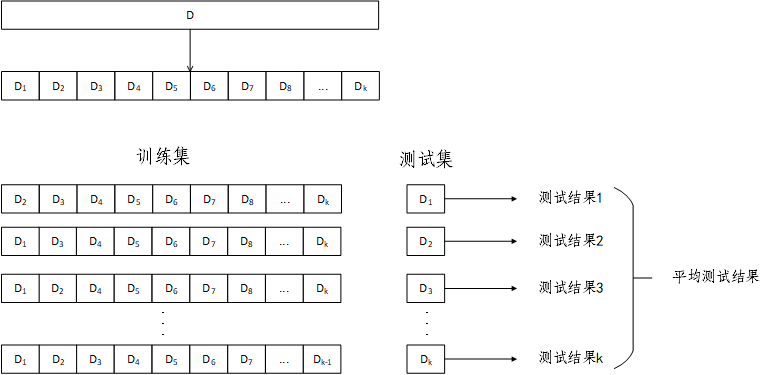
\includegraphics[width=10cm]{crossva.png}\\
  \caption{{\fangsong $k$阶交叉验证法}}
\end{figure}

\subsection{贝叶斯分类器}

对于分类任务,贝叶斯分类器基于后验概率来选择最优的类别标记。设有$N$种可能的类别,每个类别为$c_{i}$,类别集合$C=\{c_{1},c_{2},...,c_{N}\}$.给定样本$\bm{x}$,设$\bm{x}$ 属于类别$c_{i}$ 的概率为$P(c_{i}|\bm{x})$。 为了使每个样本的分类错误率最小,应该将$\bm{x}$分到使得后验概率$P(c_{i}|\bm{x})$最大的$c_{i}$ 中。

即$\bm{x}$所属的类别 $$c=\mathop{\arg\max}_{c\in C}P(c|\bm{x})$$

所以,为了达到分类错误率最小,要获得后验概率$P(c|\bm{x})$,基于贝叶斯定理
$$P(c|\bm{x})=\frac{P(c)P(\bm{x}|c)}{P(\bm{x})}$$

因为概率$P(\bm{x})$与类别$c$无关,使$P(c)P(\bm{x}|c)$达到最大值的$c$即为使后验概率$P(c|\bm{x})$达到最大值的$c$,
即
$$c=\mathop{\arg\max}_{c\in C}P(c)P(\bm{x}|c)$$

所以问题转化为了根据训练数据$D$估计先验概率$P(c)$ 和类条件概率$P(\bm{x}|c)$。 根据大数定律,$P(c)$可以通过计算各类样本出现的频率来进行估计,而估计类条件概率$P(\bm{x}|c)$需要样本$\bm{x}$所有属性的联合概率,难度较大.

\subsubsection{朴素贝叶斯分类器}

为了避开计算类条件概率$P(\bm{x}|c)$这个障碍,朴素贝叶斯分类器假设样本$\bm{x}$的所有属性$X=\{x_{1},x_{2},..,x_{d}\}$相互独立。基于此条件,有
$$P(c|\bm{x})=\frac{P(c)P(\bm{x}|c)}{P(\bm{x})}=\frac{P(c)}{P(\bm{x})}\prod_{i=1}^{d}P(x_{i}|c)$$

对于所有类别$c\in C$,$P(\bm{x})$相同,所以只需要求出使得$P(c)\prod_{i=1}^{d}P(x_{i}|c)$最大的$c$,即为$\bm{x}$的所属类别。
$$c=\mathop{\arg\max}_{c\in C}P(c)\prod_{i=1}^{d}P(x_{i}|c)$$

设$D_{c}$为训练集$D$中类别取值为$c$的样本组成的集合,$D_{c,x_{i}}$为$D$中在第$i$个属性取值为$x_{i}$,类别取值为$c$的样本组成的集合,根据大数定律,估计出类先验概率和条件概率为
$$P(c)=\frac{|D_{c}|}{|D|}$$
$$P(x_{i}|c)=\frac{|D_{c,x_{i}}|}{|D_{c}|}$$

其中,$|A|$表示有限集合$A$的元素数量.

在估计的过程中,如果第$j$个属性对应的属性值在训练集中没有出现过,即$|D_{c,x_{j}}|=0$,那么根据上述条件概率估计中$P(x_{j}|c)=0$,从而导致$P(c|\bm{x})=0$,即样本$\bm{x}$ 携带的其他属性也将失去作用。为避免这种情况的产生,采用拉普拉斯修正,
$$\hat{P}(c)=\frac{|D_{c}|+1}{|D|+N}$$
$$\hat{P}(x_{i}|c)=\frac{|D_{c,x_{i}}|+1}{|D_{c}|+N_{i}}$$

(其中$N$为训练集$D$的类别个数,$N_{i}$为第$i$个属性的取值个数)

根据修正概率,求出样本$\bm{x}$的所属类别
$$c=\mathop{\arg\max}_{c\in C}\hat{P}(c)\prod_{i=1}^{d}\hat{P}(x_{i}|c)$$

\subsubsection{树增强型朴素贝叶斯分类器}

在很多模型中,很难实现各个属性独立这个假设。树增强型朴素贝叶斯分类器关注和每个属性$x_{i}$关联性最强的父属性$px_{i}$,并假设$x_{i}$和除了$px_{i}$属性之外的其他属性都独立。
根据这个假设有
$$P(c|\bm{x})=\frac{P(c)}{P(\bm{x})}\prod_{i=1}^{d}P(x_{i}|px_{i},c)$$

因为概率$P(\bm{x})$与类别$c$无关,所以$\bm{x}$的所属类别
$$c=\mathop{\arg\max}_{c\in C}P(c)\prod_{i=1}^{d}P(x_{i}|px_{i},c)$$

为了确定任一一个属性$x_{i}$的父属性$px_{i}$,TAN算法描述如下:

1.计算任意两个属性$x_{i},x_{j}$之间的条件互信息
$$I(x_{i},x_{j}|C)=\sum_{c\in C}\sum_{x_{i}\in X}\sum_{x_{j}\in X}P(c)P(x_{i},x_{j}|c)\log \frac{P(x_{i},x_{j}|c)}{P(x_{i}|c)P(x_{j}|c)}$$.

2.以属性为节点,连接任意两个属性$x_{i}$与$x_{j}$的边的权重为$I(x_{i},x_{j}|C)$,构建加权无向图.

3.构造此加权无向图的最大生成树,并选取任意一个节点作为根节点,将每条边变为由根节点指向叶子节点的有向边.

4.加入类别节点$C$,增加从$C$到每个属性的有向边.如图2所示.
\begin{figure}[!h]
  \centering
  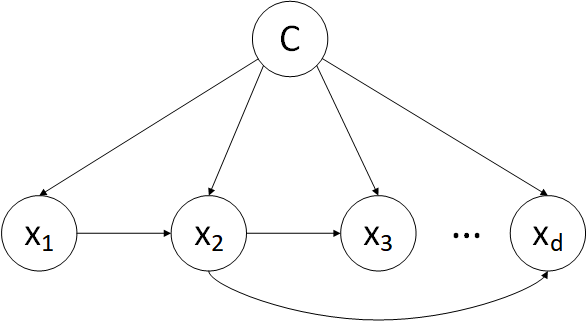
\includegraphics[width=8cm]{TAN.png}\\
  \caption{{\fangsong 最大生成树}}
\end{figure}

根据构造的最大生成树找到任意一个节点$x_{i}$的父节点$px_{i}$,并根据大数定律和拉普拉斯修正求出修正后的概率
$$\hat{P}(c)=\frac{|D_{c}|+1}{|D|+N}$$
$$\hat{P}(x_{i}|x_{j},c)=\frac{|D_{x_{i},x_{j},c}|+1}{|D_{x_{j},c}|+N_{i}}$$

(其中$D_{x_{i},x_{j},c}$为在第$i,j$个属性上取值分别为$x_{i},x_{j}$,并且类别为$c$的样本组成的集合,$N_{i}$为第$i$个属性值的取值个数)

根据修正后的概率可求出$\bm{x}$的类别
$$c=\mathop{\arg\max}_{c\in C}\hat{P}(c)\prod_{i=1}^{d}\hat{P}(x_{i}|px_{i},c)$$


\subsection{对照模型}

\subsubsection{ARIMA模型介绍}

时间序列分析方法是降水量预测方法中模型完善,精度较高的一种方法。许多学者根据时间序列分析方法对降水量预测做了大量研究。其中以ARIMA模型应用最为广泛。用此模型作为树增型朴素贝叶斯分类器的对照模型,能较好的体现出TAN分类器在降水量预测方面的表现。

建立ARIMA模型主要分3个阶段:

1.平稳性检验,纯随机性检验

对于给定的时间序列,需要检验其平稳性。非平稳序列由于样本信息太少,无法进行有效的分析。一般可以通过ADF单位根检验来判断一个时间序列的平稳性。

对于非平稳时间序列,一般采取取对数或做差分等方法,然后判断处理后的时间序列的平稳性,重复取对数或差分等操作,直到获得平稳序列。差分的次数$d$即为$\mathrm{ARIMA}(p,d,q)$ 模型中的参数$d$.

对于平稳时间序列,要进行白噪声检验。一般可以通过$Q_{LB}$统计量对序列进行检验。
$$Q_{LB}=n(n+2)\sum_{k=1}^{m}\frac{\hat{\rho}_{k}^{2}}{n-k}$$

其中,$n$为序列观测期数,$m$为指定延迟期数,$\hat{\rho}_{k}$为延迟$k$期的自相关系数估计值.

2.模型选择和参数估计

将模型ARIMA$(p,d,q)$经过差分处理转化为模型ARMA$(p,q)$.
$$X_{t}=\beta_{0}+\beta_{1}X_{t-1}+\beta_{2}X_{t-2}+\cdots+\beta_{p}X_{t-p}+\varepsilon_{t}+\alpha_{1}\varepsilon_{t-1}+\alpha_{2}\varepsilon_{t-2}+\cdots+\alpha_{q}\varepsilon_{q}$$

对于$p,q$的选择,可以根据准则AIC(Akaike Information Criterion),BIC(Bayesian Information Criterion)来确定,
当确定$p,q$的值后,可以用极大似然估计各个系数$\hat{\alpha}_{i},\hat{\beta}_{i}$和白噪声序列方差$\hat{\sigma}_{\varepsilon}^{2}$.

3.残差白噪声检验

    一个ARIMA模型的优劣可以根据一个模型是否将时间序列中的信息提取充分来判断。一个好的ARIMA模型的残差序列应该几乎不含相关信息。即残差序列应该是白噪声序列。如果不是,说明该模型对信息提取的不够充分,需要选择其他模型。可以用$Q_{LB}$统计量进行残差的白噪声检验。

4. 序列预测

     根据$p,q$的值和估计的参数,可以预测未来$n$期的值或置信区间。

\subsubsection{ BP神经网络}
       BP神经网络是人工神经网络中最常用的算法之一。其作为一种基于梯度下降法的高效的机器学习算法,具有学习能力强,能解决非线性问题等优点,在降水预测中应用较为广泛。将其作为TAN模型的对照模型,有利于对TAN模型的评估。

模型介绍:

设数据集$D$中的第$k$个样本为$(\bm{x}_{k},\bm{y}_{k})$,其中$\bm{x}_{k}=(x^{(k)}_{1},x^{(k)}_{2},...,x^{(k)}_{d})$为样本的$d$个属性,$\bm{k}_{k}=(y^{(k)}_{1},y^{(k)}_{2},..,y^{(k)}_{l})$ 为样本的$l$ 个输出值。建立一个含有$d$个输入神经元作为输入层,$q$个隐层神经元作为隐层,$l$个输出神经元作为输出层的多层前馈网络结构。神经元激活函数使用Sigmoid 函数:$$\mathrm{Sigmoid}(x)=\frac{1}{1+\mathrm{e}^{-x}}$$

并定义变量:

  \begin{table}[!h]\center\small
\begin{tabular}{|l|c|}
\hline
变量&含义\\
\hline
$\eta$ &学习率\\
\hline
$\theta_{i}$     &     输出层第$i$个神经元的阈值\\
\hline
 $\gamma_{i}$       &    隐层第$i$个神经元的阈值\\
\hline
$v_{ij}$&                 输入层第$i$个神经元与隐层第$j$个神经元连接的权重\\
\hline
$w_{ij}$&                 隐层第$i$个神经元与输出层第$j$个神经元连接的权重\\
\hline
$\alpha_{i}$&                 隐层第$i$个神经元接到的输入\\
\hline
$\beta_{i}$&                 输出层第$i$个神经元接到的输入\\
\hline
$b_{i}$&                 隐层第$i$个神经元的输出\\
\hline
$\hat{y}^{(k)}_{i}$&    数据集第$k$个样本的第$i$个预测输出值\\
\hline
$E_{k}$&                 数据集第$k$个样本的训练误差\\
\hline
$\Delta v_{ij}$&                 $v_{ij}$的更新值\\
\hline
$\Delta w_{ij}$&                 $w_{ij}$的更新值\\
\hline
$\Delta \theta_{i}$&                 $\theta_{i}$的更新值\\
\hline
$\Delta \gamma_{i}$&                 $\gamma_{i}$的更新值\\
\hline
\end{tabular}
\end{table}


算法描述:

步骤1.在(0,1)中随机初始化神经网络的连接权重和阈值

步骤2.对一个在数据集$D$中给定的样本$(\bm{x}_{k},\bm{y}_{k})$,计算神经网络的估计值$\hat{\bm{y}}_{k}$和误差$E_{k}$.
$$\alpha_{h}=\sum_{i=1}^{d}v_{ih}x^{(k)}_{i}$$
$$b_{h}=\mathrm{Sigmoid}(\alpha_{h}-\gamma_{h})$$
$$\beta_{j}=\sum_{h=1}^{q}w_{hj}b_{h}$$
$$\hat{y}_{j}^{(k)}=\mathrm{Sigmoid}(\beta_{j}-\theta_{j})$$
$$\hat{\bm{y}}_{k}=(\hat{y}_{1}^{(k)},\hat{y}_{2}^{(k)},\cdots,\hat{y}_{l}^{(k)})$$
$$E_{k}=\frac{1}{2}\sum_{j=1}^{l}(\hat{y}_{j}^{(k)}-y_{j}^{k})^{2}$$

步骤3.引入中间量$e,g$,计算阈值$\theta,\gamma$和权重$v,w$的修正值$\Delta\theta,\Delta\gamma,\Delta v,\Delta w$.
$$g_{i}=\hat{y}_{j}^{(k)}(1-\hat{y}_{j}^{(k)})(y_{j}^{(k)}-\hat{y}_{j}^{(k)})$$
$$e_{h}=b_{h}(1-b_{h})\sum_{j=1}^{l}w_{hj}g_{j}$$
$$\Delta w_{hj}=\eta g_{j}b_{h}, \ \ \ w\leftarrow w+\Delta w$$
$$\Delta\theta_{j}=-\eta g_{j},\ \ \ \theta\leftarrow \theta +\Delta \theta$$
$$\Delta v_{ih}=\eta e_{h}x^{(k)}_{i},\ \ \ v\leftarrow v+\Delta v$$
$$\Delta \gamma_{h}=-\eta e_{h},\ \ \ \gamma\leftarrow\gamma+\Delta\gamma$$

步骤4.对于所有的$(\bm{x}_{k},\bm{y}_{k})\in D$,重复步骤2,3,计算平均训练误差.
$$E=\frac{1}{|D|}\sum_{(\bm{x}_{k},\bm{y}_{k})\in D}E_{k}$$

步骤5.检查平均训练误差是否小于给定精确度,若是,输出确定的神经网络,若不是,返回步骤4.

根据上述算法,可以获得权重$v,w$和阈值$\gamma,\theta$都确定的神经网络,传入测试集的数据,即可获得预测结果。

\subsection{泛化误差评估方法}

由于贝叶斯分类器输出的是分类类型,即一个离散变量,ARIMA模型输出的是预测的具体值,BP神经网络模型输出的是(0,1)之间的实数,所以需要一个统一的方法评估几种模型的优劣。

本文采用基于二分类问题的$F$-measure方法。将预测结果分为两类,假定其中一类是``正例'',令$TP$表示实际是``正例'',分类结果也是``正例''的样本个数,$FP$表示实际不是`` 正例'',分类结果是``正例''的样本个数,$FN$表示实际是``正例'',分类结果不是``正例''的样本个数。
定义查准率$P$和查全率$R$为:
$$P=\frac{TP}{TP+FP}$$
$$R=\frac{TP}{TP+FN}$$

作为综合考察查准率和查全率的度量$F_{1}$定义为
$$F_{1}=\frac{2PR}{P+R}$$

$F_{1}$越高说明分类效果越好。


\newpage
\section{基于树增强型朴素贝叶斯分类器的实验}
\subsection{数据清洗}
   原始数据来自美国马塞纳国际机场1996年7月1日到2019年2月28日每小时记录的各项数据。由于部分数据缺失严重,在此选取10项较为完整的数据作为10项指标(日降水量,小时露点温度,小时干球温度,小时相对湿度,小时海平面气压,小时观测站气压,小时可见度,小时湿球温度,小时风向,小时风速)。整理出1996年7月到2019年2月每月的10项指标的平均值,1996年7月到2019年2月每月最后7天的10项指标的平均值。对于部分缺失值,由于直接剔除带有缺失值的数据会使得数据集变小,所以采用平均值代替缺失值的方法。


\subsection{数据降维}
因为每个月有10项指标平均值和每月最后7天的10项指标平均值,即总共有20项指标,如果不进行数据降维,将会需要大量的计算。由于20项数据的量纲不统一,采用相关系数矩阵的PCA算法,计算出相关系数矩阵的特征值,如图3所示.
\begin{figure}[!h]
  \centering
  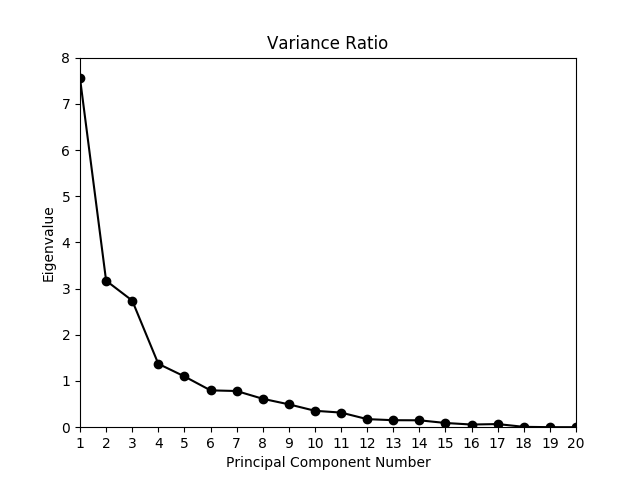
\includegraphics[width=8cm]{varRatio.png}\\
  \caption{{\fangsong 相关系数矩阵特征值}}
\end{figure}

计算出前$i$个主成分的方差所占总方差的比例:


  \begin{table}[!h]\center\footnotesize
\begin{tabular}{|l|l|l|l|}
\hline
$i$&Ratio&$i$&Ratio\\
\hline
1&0.37767&11&0.96495\\
\hline
2&0.53625&12&0.97369\\
\hline
3&0.67327&13&0.97369\\
\hline
4&0.74187&14&0.98126\\
\hline
5&0.79683&15&0.98873\\
\hline
6&0.83670&16&0.99330\\
\hline
7&0.87587&17&0.99618\\
\hline
8&0.90662&18&0.99957\\
\hline
9&0.93137&19&0.99999\\
\hline
10&0.94914&20&1.00000\\
\hline
\end{tabular}
\end{table}

由此可见,选取前7个变量即可使主成分保持信息总量的比重达到85\%以上,记这前7个主成分为$X_{0},X_{1},\cdots,X_{6}$,每个月的下个月的降水量为$C$.


\subsection{数据离散化}
朴素贝叶斯算法要求数据是分类属性形式,即要求数据是离散的。为了在离散化的同时尽可能多的保持数据原有的信息,利用Python中的pandas包,采用等频离散化的方式。将每月的7 个主成分和每月对应的下个月降水量总计8个变量进行离散化处理。用0,1,2,3,4,来表示对应数据的大小(0最小,4最大)。如下表所示:
  \begin{table}[!h]\center\scriptsize
\begin{tabular}{|l|l|l|l|l|l|}
\hline
\diagbox{主成分}{离散值}   &    0 & 1  & 2  &  3 &   4\\
\hline
$X_{0}$    &  (-38.83, -19.003] & (-19.003, -11.314] & (-11.314, -6.859] &
                                    (-6.859, -0.176] & (-0.176, 18.962]\\
                                    \hline
$X_{1}$   &  (-21.531, 4.937] & (4.937, 19.797] & (19.797, 28.056] &
                                    (28.056, 39.166] & (39.166, 73.251]\\
                                    \hline
$X_{2}$   &  (51.071, 76.059] & (76.059, 83.75] & (83.75, 90.996] &
                                    (90.996, 99.536] & (99.536, 124.049]\\
                                    \hline
$X_{3}$   & (-22.036, -8.288] & (-8.288, -1.127] & (-1.127, 7.136] &
                                    (7.136, 12.324] & (12.324, 26.037]\\
                                    \hline
$X_{4}$   & (-28.246, -17.629] & (-17.629, -10.301] & (-10.301, -4.081] &
                                    (-4.081, 3.457] & (3.457, 16.473]\\
                                    \hline
$X_{5}$    & (69.757, 84.188] & (84.188, 88.293] & (88.293, 92.095] &
                                    (92.095, 95.938] & (95.938, 111.357]\\
                                    \hline
$X_{6}$   &  (-2.723, 5.549] & (5.549, 10.251] & (10.251, 15.882] &
                                    (15.882, 22.688] &(22.688, 33.979]\\
                                    \hline
$C$ & (-0.001, 1.21] & (1.21, 2.03] & (2.03, 2.89] & (2.89, 3.95] &
                                    (3.95, 7.88]\\
                                    \hline
\end{tabular}
\end{table}

\subsection{数据分组}
   根据$k$阶交叉验证法,选取$k=5$,将数据分为5组训练集和测试集.
\subsection{TAN算法}

1.根据离散后的数据,计算任意两个属性$x_{i},x_{j}$之间的条件互信息。

\begin{table}[!h]\center\footnotesize
\begin{tabular}{|l|l|l|l|l|l|l|l|}
\hline
\diagbox{$i$}{$I(x_{i},x_{j}|c)$}{$j$}&0&1&2&3&4&5&6\\
\hline
0&2.2774 &0.4733 &0.4176 &0.9615 &0.6343 &0.3158 &0.6986 \\
\hline
1&0.4733 &2.1146 &0.427 &0.5486 &0.6577 &0.2212 &0.4996 \\
\hline
2&0.4176 &0.427 &2.3009 &0.2837 &0.2082 &0.3031 &0.2887 \\
\hline
3&0.9615 &0.5486 &0.2837 &2.1897 &0.8958 &0.2956 &1.1077 \\
\hline
4&0.6343 &0.6577 &0.2082 &0.8958 &2.1595 &0.2434 &0.9272 \\
\hline
5&0.3158 &0.2212 &0.3031 &0.2956 &0.2434 &2.2651 &0.3615 \\
\hline
6&0.6986 &0.4996 &0.2887 &1.1077 &0.9272 &0.3615 &2.156 \\
\hline
\end{tabular}
\end{table}

2.根据条件互信息计算出贝叶斯网

\begin{figure}[!h]
  \centering
  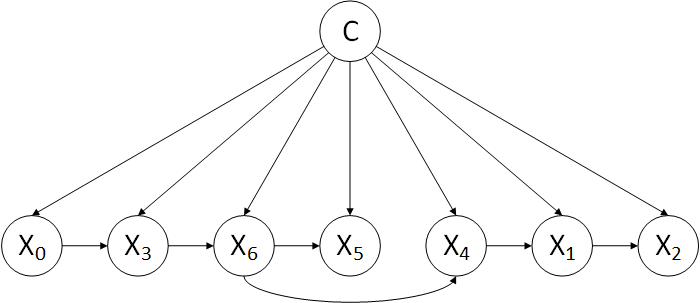
\includegraphics[width= 8cm]{BayesNet.png}\\
  \caption{{\fangsong 各个主成分和类别节点的贝叶斯网}}
\end{figure}

3.根据贝叶斯网计算测试集中样本$\bm{x}$最大后验概率$P(c|\bm{x})$对应的类别$c$,得到$\bm{x}$的分类。并与$\bm{x}$的真实类别对比,根据$F$-measure方法得到贝叶斯分类器的正确率如下表所示,可见,树增型朴素贝叶斯分类器的分类效果略优于朴素贝叶斯分类器.
\begin{table}[!h]\center\small
\begin{tabular}{|l|l|l|l|l|l|l|l|}
\hline
朴素贝叶斯 & $P$&$R$&$F_{1}$&树增型朴素贝叶斯 & $P$&$R$&$F_{1}$\\
\hline
测试集1&0.900 & 0.900 & 0.900&测试集1&0.920 & 0.821 & 0.867\\
\hline
测试集2&0.742 & 0.896 & 0.812&测试集2&0.889 & 0.923 & 0.905\\
\hline
测试集3&0.916 & 0.758 & 0.830&测试集3&0.892 & 0.862 & 0.877\\
\hline
测试集4&0.840 &0.807 & 0.823&测试集4&0.750 & 0.778 & 0.763\\
\hline
测试集5&0.857 & 0.800 & 0.827&测试集5&0.778 & 0.875 & 0.823\\
\hline
平均&0.851& 0.832& 0.841&平均&0.846& 0.851 &0.849\\
\hline
\end{tabular}
\end{table}

\newpage

\section{对比实验}
\subsection{时间序列分析}

选取1996年7月到2019年2月的月降水量作为时间序列$X_{t}$。

\subsubsection{平稳性检验和纯随机性检验}

作假设:
\newline
\indent \indent$H_{0}$:时间序列$X_{t}$非平稳.

\indent\indent$H_{1}$:时间序列$X_{t}$平稳.

利用Python的statsmodels库得到ADF单位根检验的结果:

\begin{table}[!h]\center\small
\begin{tabular}{|l|l|l|l|}
\hline
$\tau$ 统计量值 &                 -8.525&临界值(1\%)        &      -3.455\\
\hline
$p$值   &     $1.076\times 10^{-13}$&临界值(5\%)            &      -2.872\\
\hline
延迟阶数       &         6&临界值(10\%)      &        -2.572\\
\hline
\end{tabular}
\end{table}

由于$p$值显著小于0.01,所以拒绝原假设,即可以认为时间序列$X_{t}$是平稳时间序列.


作假设:
\newline
\indent\indent $H_{0}$:时间序列$X_{t}$是白噪声序列.

\indent\indent$H_{1}$:时间序列$X_{t}$不是白噪声序列

利用Python的statsmodels库,得到纯随机性检验的结果:
\begin{table}[!h]\center
\begin{tabular}{|c|c|c|}
\hline
\multirow{2}{*}{延迟}&\multicolumn{2}{|c|}{$Q_{LB}$}\\
\cline{2-3}
&$Q_{LB}$统计量值&$p$值\\
\hline
延迟6阶              &          58.192 &                  $ 1.047\times 10^{-10}$\\
\hline

延迟12阶              &              97.543         &      $ 1.683\times 10^{-15}$\\
\hline
\end{tabular}
\end{table}

由于$p$值显著小于0.01,所以拒绝原假设,即可以认为时间序列$X_{t}$不是白噪声序列.

\subsubsection{ARMA模型阶数确定和参数估计}

利用Python的statsmodels库,确定$p,q$的阶数为(4,3),模型中各个系数的极大似然估计值如下:
\begin{footnotesize}
$$X_{t}=2.613+0.980X_{t-1}+0.463X_{t-2}-1.025X_{t-3}+0.160X_{t-4}+\varepsilon_{t}-0.778\varepsilon_{t-1}-0.598\varepsilon_{t-2}+0.868\varepsilon_{t-3}$$
\end{footnotesize}
其中$\mathrm{Var}(\varepsilon_{t})=2.146$.

\subsubsection{残差白噪声检验}

作假设如下,并计算统计量$Q_{LB}$和其$p$值.
\newline
\indent\indent $H_{0}$:残差序列$Res_{t}$是白噪声序列.

\indent\indent$H_{1}$:残差序列$Res_{t}$不是白噪声序列.


\begin{table}[!htb]\center
\begin{tabular}{|c|c|c|}
\hline
\multirow{2}{*}{延迟}&\multicolumn{2}{|c|}{$Q_{LB}$}\\
\cline{2-3}
&$Q_{LB}$统计量值&$p$值\\
\hline
延迟6阶              &          0.853 &                  $ 0.990$\\
\hline

延迟12阶              &              4.684         &      $ 0.967$\\
\hline
延迟18阶              &              6.851         &      $ 0.991$\\
\hline
延迟24阶              &              11.277         &      $ 0.986$\\
\hline
\end{tabular}
\end{table}

由于$p$值显著大于0.01,所以接受原假设,认为残差序列$Res_{t}$是白噪声序列,即模型ARIMA(4,0,3)能较好的提取原时间序列的信息.


\subsubsection{预测结果}
1996年7月到2019年2月共272个月,选取前234个月作为时间序列的样本数据,后38个月作为测试数据。根据上述ARIMA(4,0,3)模型,得到测试结果如图5所示:
\begin{figure}[!h]
  \centering
  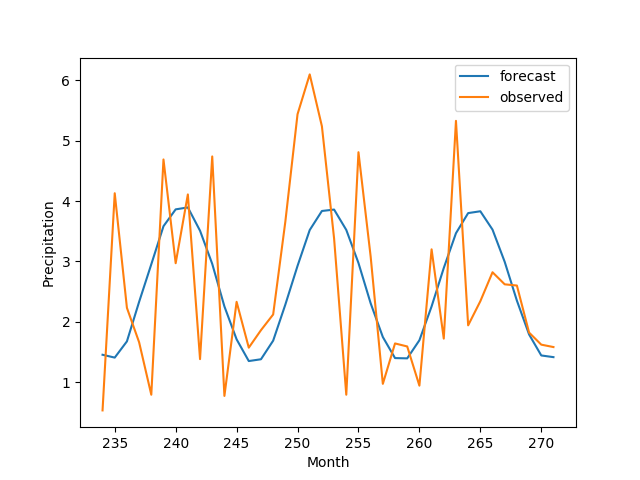
\includegraphics[width=8cm]{arima.png}\\
  \caption{{\fangsong 观测值和ARIMA模型预测值}}
\end{figure}

将观测值和预测值离散化后,得到ARMIA(4,0,3)模型的正确率

$$P= 0.730,\ \ \ R= 0.760 ,\ \ \ F_{1}= 0.745.$$

\subsection{BP神经网络}
        与TAN算法相同,先采用PCA算法进行数据降维。由于降维后的数据量纲不统一,使用min-max标准化方法将其标准化。并将标准化后的数据根据交叉验证法分为5组训练集和测试集。

选取学习率$\eta=0.01$,在迭代次数为500的情况下,通过实验模拟出当隐层神经元数量$q=10$有较好的精度和性能。

通过上文中的BP神经网络算法,计算出输出神经元的阈值$\theta$,隐层神经元的阈值$\gamma$,输入层神经元与隐层神经元的连接权重$v$,隐层神经元与输出层神经元的连接权重$w$(以第1组训练集为例).
\begin{small}
$$
 v=\left(
 \begin{matrix}
   0.55 & 1.93 & 0.23&  0.59 & 1.11 & -0.64  & 0.44 & 0.97 & 0.46  &0.55 \\
   1.72 & 0.07 & 0.31  & 0.72 & 0.87 & 0.44 &  0.28 & 0.28 & 1.01 & 0.45 \\
   -0.22 &-0.33 & 0.50 & 0.61  &0.85 & 0.54  & 0.70 & 1.10 & 0.48&  0.56\\
    0.19& -0.06 & 0.39 & 0.14 &-0.30 & 0.17& -0.12 & 0.32 & 0.77&  1.35\\
    2.15 & 1.99 & -0.06& -0.10& -0.44& -0.49  &-0.34 &  0.46&  0.19 & 0.08\\
    0.38& -1.60 & 0.47 & 0.41 & 0.39 & 0.17 &  0.17 & 0.63 &  0.73 & 0.49\\
    0.04 & 1.55 & 0.57 & 0.45&  0.75 &-0.48 &  0.44 & 0.91  & 0.71 & 0.08\\
  \end{matrix}
  \right)
$$

$$w=(-3.27,-5.71,0.71,0.64,2.20,2.00,1.71,0.85,1.20,-0.65)^{\mathrm{T}}$$

$$\theta=3.43$$

$$\gamma=(-1.01,-3.54,1.54,0.86,2.41,3.69,2.72,0.43,1.08,1.20)^{\mathrm{T}}$$

\end{small}

根据每个模型的各个参数,可以求得5组测试集的测试结果如下:

\begin{table}[!h]\center\small
\begin{tabular}{|l|l|l|l|}
\hline
BP神经网络&$P$&$R$&$F_{1}$\\
\hline
测试集1& 0.796& 1.0&  0.886\\\hline
测试集2& 0.796 &1.0&  0.886\\\hline
测试集3& 0.814 &1.0&  0.897\\\hline
测试集4 &0.703 &1.0&  0.826\\\hline
测试集5& 0.537 &1.0 & 0.698\\\hline
平均  &  0.729& 1.0 & 0.843\\\hline
\end{tabular}
\end{table}

\newpage

\section{模型评价}
由本文提出的模型和对比模型的结果,得到各个模型的泛化性能如下表:
\begin{table}[!h]\center\small
\begin{tabular}{|l|l|l|l|}
\hline
模型 &$P$&$R$&$F_{1}$\\
\hline
朴素贝叶斯&0.851& 0.832& 0.841\\\hline
树增型朴素贝叶斯&0.845& 0.851& 0.849\\\hline
ARIMA &0.730& 0.760 & 0.745\\\hline
BP神经网络 & 0.729& 1.000& 0.843\\\hline
\end{tabular}
\end{table}

可知,本文提出的基于PCA的树增型朴素贝叶斯分类器的效果要好于其他的预测方法。这说明了在经过PCA降维处理后,降低了噪声的干扰,同时,根据条件互信息构建的贝叶斯网也一定程度上避免了作出样本各个属性独立的假设而丢失部分信息。与ARIMA模型相比,本文提出的模型利用了降水时间序列之外的信息,提高了预测精度,与BP神经网络模型相比,本文提出的模型结构有结构简单,计算复杂度低,鲁棒性强的特点。

\section*{结论}
\addcontentsline{toc}{section}{结论}
   本文针对降水机理不明确,气象资料不完全的情况,提出了基于PCA的树增型朴素贝叶斯的月降水量预测模型。并通过实验数据,与常用的预测降水量的统计方法(时间序列模型,人工神经网络模型)相比,取得了较好的效果,在降水预测方面有一定的指导意义。为了提高预测准确率,应该采用贝叶斯分类器和时间序列分析相结合的方法,既考虑总体的降水趋势,又将每个月特有的信息,如气压,温度,湿度等因素考虑在内。如果需要,可与气象学方法相结合以进一步提高预测准确率。












\newpage
\begin{thebibliography}{1}
\addcontentsline{toc}{section}{参考文献}
\bibitem{1}欧善国.用能量天气学方法分析预报9405号热带风暴暴雨[J].广东气象,1995(02):34-35+25.
\bibitem{2}芮孝芳.数值天气预报的成功经验对洪水预报的启示[J].水利水电科技进展,2019,39(01):1-6.
\bibitem{3}F. Silvestro,L. Rossi,L. Campo,A. Parodi,E. Fiori,R. Rudari,L. Ferraris. Impact-based flash-flood forecasting system: Sensitivity to high resolution numerical weather prediction systems and soil moisture[J]. Journal of Hydrology,2019.

\bibitem{4}魏培培,董广涛,史军,张博文.华东地区极端降水动力降尺度模拟及未来预估[J].气候与环境研究,2019,24(01):86-104.
\bibitem{5}刘绿柳,杜良敏,廖要明,李莹,梁潇云,唐进跃,赵玉衡.基于时空统计降尺度的淮河流域夏季分月降水概率预测[J].气象,2018,44(11):1464-1470.
\bibitem{6}黎玥君,郭品文.基于BP神经网络的浙北夏季降尺度降水预报方法的应用[J].大气科学学报,2017,40(03):425-432.
\bibitem{7}黄炜,李雪真,赵嘉,赵丽华,李臣民.基于朴素贝叶斯算法的流域降水预测方法[J].水利水电科技进展,2016,36(04):65-69+79.

\bibitem{8}E.G. Ortiz-García,S. Salcedo-Sanz,C. Casanova-Mateo. Accurate precipitation prediction with support vector classifiers: A study including novel predictive variables and observational data[J]. Atmospheric Research,2014,139

\bibitem{9}奚立平,蔡文庆,吴海鹰.基于时间序列分析的无为县降水量预测模型的研究[J].安徽水利水电职业技术学院学报,2018,18(01):50-53.
\bibitem{10}孙苗,孔祥超,耿伟华.基于ARIMA模型的山东省月降水量时间序列分析[J].鲁东大学学报(自然科学版),2013,29(03):244-249.
\bibitem{11}叶晓枫,许义仿.基于Isomap的树增强朴素贝叶斯分类器的信用预测[J].中州大学学报,2017,34(06):113-116.


\bibitem{12}蒲京京,苏巧荣,张朝瑜,肖振东,吴养会.贝叶斯分类器在农村金融数据分类中的应用研究[J].安徽农学通报,2018,24(11):2-4+20.

\bibitem{13}黎月.基于贝叶斯网分类器的互联网借贷风险评估[J].北方经贸,2018(06):106-107.

\bibitem{14}杨晓君,张楠,陈宏,从靖,徐威.基于人工神经网络算法的渤海海风预报方法研究[J].干旱气象,2019,37(01):146-152.

\bibitem{15}刘攀.基于RBF和朴素贝叶斯的红葡萄酒质量等级分类[J].电子技术与软件工程,2019(04):144-145.

\bibitem{16}王妍婷.ARIMA模型在湖北省城镇居民人均消费预测中的应用[J].湖北工业职业技术学院学报,2017,30(03):67-70.

\bibitem{17}谢万里,蒲斌,王涛,尹绍武.人工神经网络在活鱼运输中水质评价的应用[J/OL].江苏农业科学:1-6[2019-03-21].

\bibitem{18}李亚军,邱润之.用时间序列方法作青岛降水、气温分析和预报[J].山东气象,1989(01):6-8.

\bibitem{19}D.A. Sachindra,K. Ahmed,Md. Mamunur Rashid,S. Shahid,B.J.C. Perera. Statistical downscaling of precipitation using machine learning techniques[J]. Atmospheric Research,2018,212.

\bibitem{20}周志华. 机器学习[M], 北京:清华大学出版社,2016.
\bibitem{20.5} Robert Sedgewick, Kevin Wayne. 算法(第四版)[M], 北京:人民邮电出版社,2012-3.


\bibitem{21}李辰飞,常婕,沈燕.ARIMA模型在湖北省GDP预测中的应用[J].湖北师范学院学报(哲学社会科学版),2015,35(04):62-66.
\bibitem{22}王燕. 应用时间序列分析(第四版)[M]. 北京: 中国人民大学出版社, 2015


\bibitem{23}何晓群. 多元统计分析(第四版)[M]. 北京: 中国人民大学出版社, 2015
\bibitem{24}杨磊磊,卢文喜,刘派,曲武.时间序列分析及Monte Carlo方法在降水预报中的应用[J].环境科学与技术,2011,34(05):108-112.
\end{thebibliography}


\newpage
\rhead{附录}
\section*{附录}
\addcontentsline{toc}{section}{附录}

\subsection*{树增型朴素贝叶斯分类器所用源程序}
\addcontentsline{toc}{subsection}{树增型朴素贝叶斯分类器所用源程序}

\subsubsection*{datacleasing.py}
\begin{scriptsize}
\begin{minted}{python}
#!/usr/bin/env python3
import csv


class DailyWeather(object):
    def __init__(self, date):
        self.date=date
        self.DPreci = 0
        self.DaDewTemp = 0
        self.NDaDewTemp = 0
        self.DaDryTemp=0
        self.NDaDryTemp=0
        self.DaRelHum=0
        self.NDaRelHum=0
        self.DaSeaLPre=0
        self.NDaSeaLPre=0
        self.DaStationPre=0
        self.NDaStationPre=0
        self.DaVisibility=0
        self.NDaVisibility=0
        self.DaWetTemp=0
        self.NDaWetTemp=0
        self.DaWindDir=0
        self.NDaWindDir=0
        self.DaWindSpeed=0
        self.NDaWindSpeed=0
        self.ifCalculate=0
        self.Date=0
        self.DailyPrecipitation=0
        self.DailyDewPointTemp=0
        self.DailyDryTemp=0
        self.DailyRelativeHumidity=0
        self.DailySeaLevelPressure=0
        self.DailyStationPressure=0
        self.DailyVisibility=0
        self.DailyWetTemp=0
        self.DailyWindDirection=0
        self.DailyWindSpeed=0

    def addDpreci(self,Dpreci):
        if Dpreci=='':
            return
        if Dpreci=='T'or Dpreci=='' or Dpreci=='Ts':
            Dpreci=0
        else:
            if Dpreci[-1]=='s':
                Dpreci=Dpreci[:-1]
            Dpreci=float(Dpreci)
        self.DPreci+=Dpreci

    def addDaDewTemp(self,DaDewTemp):
        if DaDewTemp=='' or DaDewTemp=="*":
            return
        else:
            if DaDewTemp[-1]=='s':
                DaDewTemp=DaDewTemp[:-1]
            DaDewTemp=float(DaDewTemp)
            self.DaDewTemp+=DaDewTemp
            self.NDaDewTemp+=1

    def addDaDryTemp(self,DaDryTemp):
        if DaDryTemp=='' or DaDryTemp=="*":
            return
        else:
            if DaDryTemp[-1]=='s':
                DaDryTemp=DaDryTemp[:-1]
            DaDryTemp=float(DaDryTemp)
            self.DaDryTemp+=DaDryTemp
            self.NDaDryTemp+=1

    def addDaRelHum(self,DaRelHum):
        if DaRelHum=='' or DaRelHum=="*":
            return
        else:
            if DaRelHum[-1]=='s':
                DaRelHum=DaRelHum[:-1]
            DaRelHum=float(DaRelHum)
            self.DaRelHum+=DaRelHum
            self.NDaRelHum+=1

    def addDaSeaLPre(self,DaSeaLPre):
        if DaSeaLPre=='' or DaSeaLPre=="*":
            return
        else:
            if DaSeaLPre[-1]=='s':
                DaSeaLPre=DaSeaLPre[:-1]
            DaSeaLPre=float(DaSeaLPre)
            self.DaSeaLPre+=DaSeaLPre
            self.NDaSeaLPre+=1

    def addDaStationPre(self,DaStationPre):
        if DaStationPre=='' or DaStationPre=="*":
            return
        else:
            if DaStationPre[-1]=='s':
                DaStationPre=DaStationPre[:-1]
            DaStationPre=float(DaStationPre)
            self.DaStationPre+=DaStationPre
            self.NDaStationPre+=1

    def addDaVisibility(self,DaVisibility):
        if DaVisibility=='' or DaVisibility=="*":
            return
        else:
            if DaVisibility[-1]=='V' or DaVisibility[-1]=='s':
                DaVisibility=DaVisibility[:-1]
            DaVisibility=float(DaVisibility)
            self.DaVisibility+=DaVisibility
            self.NDaVisibility+=1

    def addDaWetTemp(self,DaWetTemp):
        if DaWetTemp=='' or DaWetTemp=="*":
            return
        else:
            if DaWetTemp[-1]=='s':
                DaWetTemp=DaWetTemp[:-1]
            DaWetTemp=float(DaWetTemp)
            self.DaWetTemp+=DaWetTemp
            self.NDaWetTemp+=1

    def addDaWindDir(self,DaWindDir):
        if DaWindDir=='' or DaWindDir=="VRB":
            return
        else:
            if DaWindDir[-1]=='s':
                DaWindDir=DaWindDir[:-1]
            DaWindDir=float(DaWindDir)
            self.DaWindDir+=DaWindDir
            self.NDaWindDir+=1

    def addDaWindSpeed(self,DaWindSpeed):
        if DaWindSpeed=='' or DaWindSpeed=="VRB":
            return
        else:
            if DaWindSpeed[-1]=='s':
                DaWindSpeed=DaWindSpeed[:-1]
            DaWindSpeed=float(DaWindSpeed)
            self.DaWindSpeed+=DaWindSpeed
            self.NDaWindSpeed+=1

    def calculate(self):
        self.Date=self.date
        self.DailyPrecipitation=self.DPreci
        self.DailyDewPointTemp="No data" if self.NDaDryTemp==0 else self.DaDewTemp/self.NDaDryTemp
        self.DailyDryTemp="No data"if self.NDaDryTemp==0 else self.DaDryTemp/self.NDaDryTemp
        self.DailyRelativeHumidity="No data"if self.NDaRelHum==0 else self.DaRelHum/self.NDaRelHum
        self.DailySeaLevelPressure="No data"if self.NDaSeaLPre==0 else self.DaSeaLPre/self.NDaSeaLPre
        self.DailyStationPressure="No data" if self.NDaStationPre==0 else self.DaStationPre/self.NDaStationPre
        self.DailyVisibility="No data"if self.NDaVisibility==0 else self.DaVisibility/self.NDaVisibility
        self.DailyWetTemp="No data"if self.NDaWetTemp==0 else self.DaWetTemp/self.NDaWetTemp
        self.DailyWindDirection="No data" if self.NDaWindDir==0 else self.DaWindDir/self.NDaWindDir
        self.DailyWindSpeed="No data" if self.NDaWindSpeed==0 else self.DaWindSpeed/self.NDaWindSpeed
        self.ifCalculate=1

    def print(self):
        if self.ifCalculate==0:
            raise ValueError("uncalculated data in "+self.date+"!")
        print('Date=',self.Date)
        print('DailyPrecipitation=',self.DPreci)
        print('DailyDewPointTemp=',self.DailyDewPointTemp)
        print('DailyDryTemp=',self.DailyDryTemp)
        print('DailyRelativeHumidity=',self.DailyRelativeHumidity)
        print('DailySeaLevelPressure=',self.DailySeaLevelPressure)
        print('DailyStationPressure=',self.DailyStationPressure)
        print('DailyVisibility=',self.DailyVisibility)
        print('DailyWetTemp=',self.DailyWetTemp)
        print('DailyWindDirection=',self.DailyWindDirection)
        print('DailyWindSpeed=',self.DailyWindSpeed)

    def add(self,wholedata):
        self.addDpreci(wholedata[3])
        self.addDaDewTemp(wholedata[5])
        self.addDaDryTemp(wholedata[6])
        self.addDaRelHum(wholedata[7])
        self.addDaSeaLPre(wholedata[8])
        self.addDaStationPre(wholedata[9])
        self.addDaVisibility(wholedata[10])
        self.addDaWetTemp(wholedata[11])
        self.addDaWindDir(wholedata[12])
        self.addDaWindSpeed(wholedata[13])


class MonthlyWeather(object):
    def __init__(self,month):
        self.month=month
        self.Day=[]
        self.data30=[0,]*10
        self.count30=[0,]*10
        self.data7=[0,]*10
        self.count7=[0,]*10

    def calculate7(self):
        day7=self.Day[-7:]
        for i in day7:
            if i.ifCalculate == 0:
                raise ValueError("uncalculated data in " + i.date + "!")
            if i.DailyPrecipitation!="No data":
                self.data7[0]+=i.DailyPrecipitation
                self.count7[0]=1
            if i.DailyDewPointTemp != "No data":
                self.data7[1] += i.DailyDewPointTemp
                self.count7[1] += 1
            if i.DailyDryTemp != "No data":
                self.data7[2] += i.DailyDryTemp
                self.count7[2] += 1
            if i.DailyRelativeHumidity != "No data":
                self.data7[3] += i.DailyRelativeHumidity
                self.count7[3] += 1
            if i.DailySeaLevelPressure != "No data":
                self.data7[4] += i.DailySeaLevelPressure
                self.count7[4] += 1
            if i.DailyStationPressure != "No data":
                self.data7[5] += i.DailyStationPressure
                self.count7[5] += 1
            if i.DailyVisibility != "No data":
                self.data7[6] += i.DailyVisibility
                self.count7[6] += 1
            if i.DailyWindDirection != "No data":
                self.data7[7] += i.DailyWindDirection
                self.count7[7] += 1
            if i.DailyWindSpeed != "No data":
                self.data7[8] += i.DailyWindSpeed
                self.count7[8] += 1
            if i.DailyWetTemp != "No data":
                self.data7[9] += i.DailyWetTemp
                self.count7[9] += 1
        for i in range(len(self.data7)):
            if self.count7[i]==0:
                self.data7[i]="No data"
            else:
                self.data7[i]/=self.count7[i]

    def calculate30(self):
        day30=self.Day[:]
        for i in day30:
            if i.ifCalculate == 0:
                raise ValueError("uncalculated data in " + i.date + "!")
            if i.DailyPrecipitation!="No data":
                self.data30[0]+=i.DailyPrecipitation
                self.count30[0]=1
            if i.DailyDewPointTemp != "No data":
                self.data30[1] += i.DailyDewPointTemp
                self.count30[1] += 1
            if i.DailyDryTemp != "No data":
                self.data30[2] += i.DailyDryTemp
                self.count30[2] += 1
            if i.DailyRelativeHumidity != "No data":
                self.data30[3] += i.DailyRelativeHumidity
                self.count30[3] += 1
            if i.DailySeaLevelPressure != "No data":
                self.data30[4] += i.DailySeaLevelPressure
                self.count30[4] += 1
            if i.DailyStationPressure != "No data":
                self.data30[5] += i.DailyStationPressure
                self.count30[5] += 1
            if i.DailyVisibility != "No data":
                self.data30[6] += i.DailyVisibility
                self.count30[6] += 1
            if i.DailyWindDirection != "No data":
                self.data30[7] += i.DailyWindDirection
                self.count30[7] += 1
            if i.DailyWindSpeed != "No data":
                self.data30[8] += i.DailyWindSpeed
                self.count30[8] += 1
            if i.DailyWetTemp != "No data":
                self.data30[9] += i.DailyWetTemp
                self.count30[9] += 1
        for i in range(len(self.data30)):
            if self.count30[i]==0:
                self.data30[i]="No data"
            else:
                self.data30[i]/=self.count30[i]

    def print(self):
        print("Month:=",self.month)
        print("Precipitation=",self.data30[0],self.data7[0])
        print("DewTemperature=",self.data30[1],self.data7[1])
        print("DryBulbTemperature=",self.data30[2],self.data7[2])
        print("RelativeHumidity=",self.data30[3],self.data7[3])
        print("SeaLevelPressure=",self.data30[4],self.data7[4])
        print("StationPressure=",self.data30[5],self.data7[4])
        print("Visibility=",self.data30[6],self.data7[6])
        print("WindDirection=",self.data30[7],self.data7[7])
        print("WindSpeed=",self.data30[8],self.data7[8])
        print("WetBulbTemperature=",self.data30[9],self.data7[9])


def getDailyWeather():
    data = []
    with open('WeatherData1996To1999.csv', 'r') as f:
        file = csv.reader(f)
        for item in file:
            data.append(item)
    with open('WeatherData2000To2009.csv', 'r') as f:
        file = csv.reader(f)
        for item in file:
            data.append(item)
    with open('WeatherData2010To2019.csv', 'r') as f:
        file = csv.reader(f)
        for item in file:
            data.append(item)
    dic = {}
    for i in data:
        if i[0] == 'DATE':
            continue
        date = i[0].split('T')[0]
        if date in dic.keys():
            continue
        dic.update({date: DailyWeather(date)})
    for i in data:
        if i[0] == 'DATE':
            continue
        date = i[0].split('T')[0]
        dic[date].add(i)
    for i in dic.keys():
        dic[i].calculate()
    return dic


def writeDailyWeather():
    dic=getDailyWeather()
    with open('DailyWeather.txt', 'w',newline='') as f:
        file = csv.writer(f)
        csv_in=[]
        csv_in.append('Date')
        csv_in.append('DailyPrecipitation')
        csv_in.append('DailyDewPointTemperature')
        csv_in.append('DailyDryBulbTemperature')
        csv_in.append('DailyRelativeHumidity')
        csv_in.append('DailySeaLevelPressure')
        csv_in.append('DailyStationPressure')
        csv_in.append('DailyVisibility')
        csv_in.append('DailyWetBulbTemperature')
        csv_in.append('DailyWindDirection')
        csv_in.append('DailyWindSpeed')
        file.writerow(csv_in)
        for i in dic.keys():
            csv_in = []
            csv_in.append(dic[i].Date)
            csv_in.append(dic[i].DailyPrecipitation)
            csv_in.append(dic[i].DailyDewPointTemp)
            csv_in.append(dic[i].DailyDryTemp)
            csv_in.append(dic[i].DailyRelativeHumidity)
            csv_in.append(dic[i].DailySeaLevelPressure)
            csv_in.append(dic[i].DailyStationPressure)
            csv_in.append(dic[i].DailyVisibility)
            csv_in.append(dic[i].DailyWetTemp)
            csv_in.append(dic[i].DailyWindDirection)
            csv_in.append(dic[i].DailyWindSpeed)
            file.writerow(csv_in)


def getAverage(monthlyDic):
    aver30=[0,]*10
    Naver30=[0,]*10
    aver7=[0,]*10
    Naver7=[0,]*10
    for i in monthlyDic.values():
        for j in range(10):
            if i.data7[j]!="No data":
                aver7[j]+=i.data7[j]
                Naver7[j]+=1
            if i.data30[j]!="No data":
                aver30[j]+=i.data30[j]
                Naver30[j]+=1
    for i in range(10):
        aver7[i]/=Naver7[i]
        aver30[i]/=Naver30[i]
    for i in monthlyDic.values():
        for j in range(10):
            if i.data7[j]=="No data":
                i.data7[j]=aver7[j]
            if i.data30[j]=="No data":
                i.data30[j]=aver30[j]


def getMonthlyWeather():
    dic=getDailyWeather()
    MonthlyDic = {}
    for i in dic.keys():
        splt=i.split("-")
        date = splt[0]+"-"+splt[1]
        if date in MonthlyDic.keys():
            continue
        MonthlyDic.update({date: MonthlyWeather(date)})
    for i in dic.values():
        idate=i.date.split("-")[0]+"-"+i.date.split("-")[1]
        MonthlyDic[idate].Day.append(i)
    for i in MonthlyDic.values():
        i.calculate7()
        i.calculate30()
    getAverage(MonthlyDic)
    return MonthlyDic

def writeMonthlyWeather():
    dic=getMonthlyWeather()
    with open('MonthlyWeather.txt', 'w',newline='') as f:
        file = csv.writer(f)
        csv_in=[]
        csv_in.append('Month')
        csv_in.append('MonthlyTotallyPrecipitation')
        csv_in.append('MonthlyAverageDewPointTemperature')
        csv_in.append('MonthlyAverageDryBulbTemperature')
        csv_in.append('MonthlyAverageRelativeHumidity')
        csv_in.append('MonthlyAverageSeaLevelPressure')
        csv_in.append('MonthlyAverageStationPressure')
        csv_in.append('MonthlyAverageVisibility')
        csv_in.append('MonthlyAverageWindDirection')
        csv_in.append('MonthlyAverageWindSpeed')
        csv_in.append('MonthlyAverageWetBulbTemperature')
        csv_in.append('MonthlyLast7DaysAveragePrecipitation')
        csv_in.append('MonthlyLast7DaysAverageDewPointTemperature')
        csv_in.append('MonthlyLast7DaysAverageDryBulbTemperature')
        csv_in.append('MonthlyLast7DaysAverageRelativeHumidity')
        csv_in.append('MonthlyLast7DaysAverageSeaLevelPressure')
        csv_in.append('MonthlyLast7DaysAverageStationPressure')
        csv_in.append('MonthlyLast7DaysAverageVisibility')
        csv_in.append('MonthlyLast7DaysAverageWindDirection')
        csv_in.append('MonthlyLast7DaysAverageWindSpeed')
        csv_in.append('MonthlyLast7DaysAverageWetBulbTemperature')
        file.writerow(csv_in)
        for i in dic.values():
            csv_in=[]
            csv_in.append(i.month)
            for e in i.data30:
                csv_in.append(e)
            for e in i.data7:
                csv_in.append(e)
            file.writerow(csv_in)


if __name__=="__main__":
    writeDailyWeather()
    writeMonthlyWeather()

\end{minted}
\end{scriptsize}

\subsubsection*{pca.py}
\begin{scriptsize}
\begin{minted}{python}
#!/usr/bin/env python3
import numpy as np
import matplotlib.pyplot as plt


def PCA(dataArray):
    dataArray=dataArray.T
    corr=np.corrcoef(dataArray)
    (A,B)=np.linalg.eig(corr)
    return A,B


def showPic(dataArray):
    A, B = PCA(dataArray)
    ratio = 0
    for i in range(len(A)):
        ratio += A[i] / sum(A)
        print(round(ratio, 5))
    x = []
    for i in range(1, 21):
        x.append(i)
    plt.xticks(x)
    plt.plot(x, A, color='black', marker='o')
    plt.xlim(1, 20)
    plt.ylim(0, 8)
    plt.xlabel("Principal Component Number")
    plt.ylabel("Eigenvalue")
    plt.title("Variance Ratio")
    plt.show()


if __name__=="__main__":
    a=np.loadtxt('MonthlyWeather.txt',delimiter=',')
    A, B = PCA(a)
    showPic(a)
    P=B[0:7]
    C=np.dot(P,a.T)
    np.savetxt('dataAfterPCA.txt',C,delimiter=' ')

\end{minted}
\end{scriptsize}
\subsubsection*{dataPlusPreci.py}
\begin{scriptsize}
\begin{minted}{python}
#!/usr/bin/env python3
import csv
import numpy as np


if __name__=="__main__":
    data=[]
    with open('MonthlyWeather.csv','r') as f:
        file=csv.reader(f)
        for i in file:
            data.append(i)
    m=np.size(data,0)
    n=np.size(data,1)
    precipitation=[]
    for i in range(1,m):
        precipitation.append(float(data[i][1]))
    precipitation=precipitation[1:]
    a=np.loadtxt('dataAfterPCA.txt')
    b=np.delete(a,271,axis=1)
    b=np.row_stack((b,precipitation))
    np.savetxt('dataPlusPrecipitation.txt',b)

\end{minted}
\end{scriptsize}
\subsubsection*{discretization.py}
\begin{scriptsize}
\begin{minted}{python}
#!/usr/bin/env python3
import pandas as pd
import numpy as np


if __name__=="__main__":
    data=pd.read_csv('dataPlusPrecipitation.txt',header=None,sep=' ')
    for j in range(8):
        vect=data.iloc[j]
        c=pd.qcut(vect,5,labels=[0,1,2,3,4])
        for i in range(len(vect)):
            pass
            data[i][j]=c[i]
    data=data.values
    np.savetxt('dataAfterDiscrete.txt',data)
\end{minted}
\end{scriptsize}


\subsubsection*{dataDivision.py}
\begin{scriptsize}
\begin{minted}{python}
#!/usr/bin/env python3
import numpy as np


if __name__=="__main__":
    b=np.loadtxt('dataAfterDiscrete.txt')
    step=54
    for i in range(5):
        begin=i*step
        end=(i+1)*step
        test=b[:,begin:end]
        train=np.delete(b,range(begin,end),axis=1)
        np.savetxt('Test{}.txt'.format(i),test)
        np.savetxt('Training{}.txt'.format(i),train)
\end{minted}
\end{scriptsize}

\subsubsection*{CMI.py}
\begin{scriptsize}
\begin{minted}{python}
#!/usr/bin/env python3
import numpy as np
import math


class CMI(object):
    def __init__(self,data,cmi1,cmi2):
        self.data=data
        self.cmi1=cmi1
        self.cmi2=cmi2
        self.m=np.size(data,1)

    def N(self,xi,xj,c):
        n=0
        for k in range(self.m):
            if self.data[7][k]==c and self.data[self.cmi1][k]==xi:
                if self.data[self.cmi2][k]==xj:
                    n+=1
        return n

    def N1(self,xi,c):
        n=0
        for k in range(self.m):
            if self.data[7][k]==c and self.data[self.cmi1][k]==xi:
                n+=1
        return n

    def N2(self,xj,c):
        n=0
        for k in range(self.m):
            if self.data[7][k]==c and self.data[self.cmi2][k]==xj:
                n+=1
        return n

    def Nc(self,c):
        n = 0
        for k in range(self.m):
            if self.data[7][k] == c:
                n += 1
        return n

    def Cmi(self):
        I=0
        for i in range(5):
            for j in range(5):
                for k in range(5):
                    P_xi_xj_c=self.N(i,j,k)/self.m
                    P_c=self.Nc(k)/self.m
                    P_xi_c=self.N1(i,k)/self.m
                    P_xj_c=self.N2(j,k)/self.m
                    if P_xi_xj_c==0 or P_xj_c==0 or P_xi_c==0:
                        info=0
                    else:
                        fac=(P_c*P_xi_xj_c)/(P_xi_c*P_xj_c)
                        info=P_xi_xj_c*math.log(fac,2)
                    I+=info
        return I


if __name__=="__main__":
    data=np.loadtxt('dataAfterDiscrete.txt')
    cinfo=np.zeros((7,7))
    for i in range(7):
        for j in range(7):
            cmi=CMI(data,i,j)
            cinfo[i][j]=cmi.Cmi()
    np.savetxt('MutualInformation.txt',cinfo,delimiter=',')
    for i in range(7):
        print('{',end='')
        for j in range(7):
            s=',' if j<6 else ''
            print("{}{}".format(round(cinfo[i][j],4),s),end='')
        print('}')

\end{minted}
\end{scriptsize}
\subsubsection*{PrimMST.java}
\begin{scriptsize}
\begin{minted}{java}
import java.util.LinkedList;
import java.util.PriorityQueue;
import java.util.Queue;
import java.util.Stack;

public class PrimMST
{
    private boolean[] marked;
    private Queue<Edge> mst;
    private PriorityQueue<Edge> pq;

    public PrimMST(EdgeWeightedGraph G)
    {
        pq=new PriorityQueue<>();
        marked=new boolean[G.V()];
        mst=new LinkedList<>();
        visit(G,0);
        while(!pq.isEmpty())
        {
            Edge e=pq.poll();
            int v=e.either(),w=e.other(v);
            if(marked[v]&&marked[w])
                continue;
            mst.offer(e);
            if(!marked[v]) visit(G,v);
            if(!marked[w]) visit(G,w);
        }
    }

    private void visit(EdgeWeightedGraph G,int v)
    {
        marked[v]=true;
        for(Edge e:G.adj(v))
        {
            if(!marked[e.other(v)])
                pq.add(e);
        }
    }

    public Iterable<Edge> edges()
    {
        return mst;
    }

    public double weight()
    {
        double weight=0;
        for(Edge i:edges())
        {
            weight+=i.weight();
        }
        return weight;
    }

    public static void main(String[] args)
    {
        double[][] cmi=new double[7][7];
        cmi[0]=new double[]{2.2774,0.4733,0.4176,0.9615,0.6343,0.3158,0.6986};
        cmi[1]=new double[]{0.4733,2.1146,0.427,0.5486,0.6577,0.2212,0.4996};
        cmi[2]=new double[]{0.4176,0.427,2.3009,0.2837,0.2082,0.3031,0.2887};
        cmi[3]=new double[]{0.9615,0.5486,0.2837,2.1897,0.8958,0.2956,1.1077};
        cmi[4]=new double[]{0.6343,0.6577,0.2082,0.8958,2.1595,0.2434,0.9272};
        cmi[5]=new double[]{0.3158,0.2212,0.3031,0.2956,0.2434,2.2651,0.3615};
        cmi[6]=new double[]{0.6986,0.4996,0.2887,1.1077,0.9272,0.3615,2.156};

        EdgeWeightedGraph G=new EdgeWeightedGraph(7);
        for(int i=0;i<7;++i)
        {
            for(int j=0;j<i;++j)
            {
                G.addEdge(new Edge(i,j,-cmi[i][j]));
            }
        }
        PrimMST pmst=new PrimMST(G);
        for(Edge i:pmst.edges())
        {
            System.out.println(i);
        }

    }
}

class Edge implements Comparable<Edge>
{
    private final int v;
    private final int w;
    private final double weight;
    public Edge(int v,int w,double weight)
    {
        this.v=v;
        this.w=w;
        this.weight=weight;
    }
    public double weight()
    {
        return weight;
    }
    public int either()
    {
        return v;
    }
    public int other(int vertex)
    {
        if(vertex==this.v)
            return w;
        else if(vertex==this.w)
            return v;
        else throw new RuntimeException("Inconsistent edge");
    }
    @Override
    public int compareTo(Edge that)
    {
        if(this.weight<that.weight)
            return -1;
        else if(this.weight>that.weight)
            return 1;
        else return 0;
    }
    @Override
    public String toString()
    {
        return String.format("%d--%d %.2f",v,w,weight);
    }
}

class EdgeWeightedGraph
{
    private final int V;
    private int E;
    private Stack<Edge>[] adj;
    public EdgeWeightedGraph(int V)
    {
        this.V=V;
        this.E=0;
        adj=(Stack<Edge>[]) new Stack[V];
        for(int i=0;i<V;++i)
        {
            adj[i]=new Stack<>();
        }
    }
    public int V()
    {
        return V;
    }
    public int E()
    {
        return E;
    }
    public void addEdge(Edge e)
    {
        int v=e.either(),w=e.other(v);
        adj[v].add(e);
        adj[w].add(e);
        ++E;
    }
    public Iterable<Edge> adj(int v)
    {
        return adj[v];
    }
    public Iterable<Edge> edges()
    {
        Stack<Edge> b=new Stack<>();
        for(int i=0;i<V;++i)
        {
            for(Edge e:adj[i])
            {
                if(e.other(i)>i)
                    b.add(e);
            }
        }
        return b;
    }
    @Override
    public String toString()
    {
        String s=V+" vertices, "+E+"edges\n";
        for(int v=0;v<V;++v)
        {
            s+=v+": ";
            for(Edge w:adj(v))
            {
                s+=w+" ";
            }
            s+="\n";
        }
        return s;
    }
}

\end{minted}
\end{scriptsize}
\subsubsection*{Bayes.py}
\begin{scriptsize}
\begin{minted}{python}
#!/usr/bin/env python3
import numpy as np
from math import log
from TAN.CMI import CMI


class Prediction(object):
    def __init__(self,train,test):
        self.train=train
        self.test=test
        self.parray=[]
        self.clas=0
        for c in range(5):
            self.parray.append(self.Naiveprob(c))
        self.logp=self.parray[0]
        for i in range(1,len(self.parray)):
            if self.parray[i]>self.logp:
                self.logp=self.parray[i]
                self.clas=i

    def P_xi_pxi_c(self,xi,pxi,xi_value,pxi_value,c):
        cmi=CMI(self.train,xi,pxi)
        a=cmi.N(xi_value,pxi_value,c)+1
        b=cmi.N2(pxi_value,c)+5
        return a/b

    def P_x0_c(self,x0,x0_value,c):
        cmi=CMI(self.train,x0,1)
        a=cmi.N1(x0_value,c)+1
        b=cmi.Nc(c)+5
        return a/b

    def P_c(self,c):
        cmi=CMI(self.train,0,1)
        a=cmi.Nc(c)
        b=np.size(train,1)
        return a/b

    def prob(self,c):
        p53=self.P_xi_pxi_c(5,6,self.test[5],self.test[6],c)
        p36=self.P_xi_pxi_c(2,1,self.test[2],self.test[1],c)
        p26=self.P_xi_pxi_c(1,4,self.test[1],self.test[4],c)
        p60=self.P_xi_pxi_c(4,6,self.test[4],self.test[6],c)
        p14=self.P_xi_pxi_c(6,3,self.test[6],self.test[3],c)
        p40=self.P_xi_pxi_c(3,0,self.test[3],self.test[0],c)
        p0=self.P_x0_c(0,self.test[0],c)
        pc=self.P_c(c)
        p=log(pc)+log(p53)+log(p36)+log(p26)+log(p60)+log(p14)+log(p40)+log(p0)
        return p

    def Naiveprob(self,c):
        p=0
        for i in range(7):
            p+=log(self.P_x0_c(i,self.test[i],c))
        p+=log(self.P_c(c))
        return p


if __name__=="__main__":
    for s in range(5):
        train=np.loadtxt('Training{}.txt'.format(s))
        tes=np.loadtxt('Test{}.txt'.format(s))
        tp=0
        tn=0
        fp=0
        fn=0
        P=R=F1=0
        for i in range(np.size(tes,1)):
            t=tes[:,i]
            s=Prediction(train,t)
            if s.clas<3 and t[7]<3:
                tp+=1
            if s.clas<3 and t[7]>3:
                fp+=1
            if s.clas>3 and t[7]<3:
                fn+=1
            if s.clas>3 and t[7]>3:
                tn+=1
        P=tp/(tp+fp)
        R=tp/(tp+fn)
        F1=2*P*R/(P+R)
        print('P=',P,',R=',R,',F1=',F1)

\end{minted}
\end{scriptsize}


\subsection*{ARIMA模型所用源程序}
\addcontentsline{toc}{subsection}{ARIMA模型所用源程序}

\subsubsection*{precheck.py}
\begin{scriptsize}
\begin{minted}{python}
#!/usr/bin/env python3
import pandas as pd
import statsmodels.tsa.stattools as ts
from statsmodels.sandbox.stats.diagnostic import acorr_ljungbox

if __name__=="__main__":
    allData=pd.read_csv('MonthlyWeather.txt',header=None,sep=',')
    data=allData.iloc[:,0]
    print(ts.adfuller(data,autolag='AIC'))
    p_value = acorr_ljungbox(data,lags=[6,12])
    print(p_value)
\end{minted}
\end{scriptsize}

\subsubsection*{arima.py}
\begin{scriptsize}
\begin{minted}{python}
#!/usr/bin/env python3
import pandas as pd
import numpy as np
import statsmodels.tsa.stattools as st
from statsmodels.tsa.arima_model import ARMA
from statsmodels.sandbox.stats.diagnostic import acorr_ljungbox
import matplotlib.pyplot as plt

if __name__=="__main__":
    allData=pd.read_csv('MonthlyWeather.txt',header=None,sep=',')
    data=allData.iloc[:,0]
    original_new=data[234:]
    data=data[0:234]
    order = st.arma_order_select_ic(data,ic=['aic', 'bic'])
    model = ARMA(data, order=(4,3))
    result_arma = model.fit(disp=-1,method='css')
    print(result_arma.summary())
    predict_ts = result_arma.predict()
    err=(data-predict_ts).dropna()
    p_value = acorr_ljungbox(err,[6,12,18,24])
    print(p_value)
    predict_new=result_arma.predict(234,271,)
    ax=predict_new.plot(label='forecast')
    original_new.plot(label='observed')
    ax.set_xlabel('Month')
    ax.set_ylabel('Precipitation')
    plt.legend()
    plt.show()
    predict_new=predict_new.values
    original_new=original_new.values
    tp=0
    tn=0
    fp=0
    fn=0
    threshold=3.94
    P=R=F1=0
    for i in range(np.size(predict_new)):
        if predict_new[i]<3 and original_new[i]<3:
            tp+=1
        if predict_new[i]<3 and original_new[i]>3:
            fp+=1
        if predict_new[i]>3 and original_new[i]<3:
            fn+=1
        if predict_new[i]>3 and original_new[i]>3:
            tn+=1
    P=tp/(tp+fp)
    R=tp/(tp+fn)
    F1=2*P*R/(P+R)
    print('P=',P,',R=',R,',F1=',F1)
\end{minted}
\end{scriptsize}












\subsection*{BP神经网络模型所用源程序}
\addcontentsline{toc}{subsection}{BP神经网络模型所用源程序}
\subsubsection*{BP.py}
\begin{scriptsize}
\begin{minted}{python}
import numpy as np


def sigmoid(x):
    return 1/(1+np.exp(-x))


def datadivision(In):
    b = np.loadtxt(In)
    step = 54
    for i in range(5):
        begin = i * step
        end = (i + 1) * step
        test = b[:, begin:end]
        train = np.delete(b, range(begin, end), axis=1)
        np.savetxt('Test{}.txt'.format(i), test)
        np.savetxt('Training{}.txt'.format(i), train)


def standardize(In,Out):
    data = np.loadtxt(In)
    m, n = np.size(data, 0), np.size(data, 1)
    for i in range(m):
        for j in range(n):
            data[i][j] = (data[i][j] - data[i].min()) / (data[i].max()-data[i].min())
    np.savetxt(Out, data)
    return data[7].mean(),data[7].std()


def BPNeutualNetwork(database,d,q,l,eta,iteration_number=500):
    D=database
    theta = np.random.rand(l, 1)
    gamma = np.random.rand(q,1)
    v = np.random.rand(d, q)
    w = np.random.rand(q, l)
    alpha = np.zeros(q)
    beta = np.zeros(l)
    b = np.zeros(q)
    y_estimate = np.zeros(l)
    E = 0
    g = np.zeros(l)
    for iteration in range(iteration_number):
        E = 0
        for column in range(np.size(D, 1)):
            x = D[:-1, column]
            y = D[-1][column]
            for i in range(np.size(v, 1)):
                alpha[i] = np.array(v[:, i]).dot(x)
            for h in range(np.size(b)):
                b[h]=sigmoid(alpha[h]-gamma[h])
            for i in range(np.size(w, 1)):
                beta[i] = np.array(w[:, i]).dot(b)
            y_estimate = sigmoid(beta - theta)
            E += 0.5 * (y_estimate - y).dot(y_estimate - y)
            g = y_estimate * (1 - y_estimate) * (y - y_estimate)
            w_delta = np.zeros((q, l))
            for i in range(np.size(b)):
                for j in range(np.size(g)):
                    w_delta[i][j] = eta * b[i] * g[j]
            theta_delta = np.zeros(np.size(theta))
            for j in range(np.size(g)):
                theta_delta[j] = -eta * g[j]
            e = np.zeros(np.size(b))
            sumh = np.zeros(np.size(b))
            for h in range(np.size(sumh)):
                for j in range(l):
                    sumh[h] += w[h][j] * g[j]
            e = b * (1 - b) * sumh
            v_delta = np.zeros((d, q))
            for i in range(np.size(x)):
                for h in range(np.size(e)):
                    v_delta[i][h] = eta * e[h] * x[i]
            gamma_delta = np.zeros((q, 1))
            for h in range(np.size(e)):
                gamma_delta[h] = -eta * e[h]
            w += w_delta
            theta += theta_delta
            v += v_delta
            gamma += gamma_delta
        E /= np.size(D, 1)
    return theta,gamma,v,w,E


def calculate(Testdata,v,w,theta,gamma):
    D=Testdata
    alpha = np.zeros(q)
    beta = np.zeros(l)
    b = np.zeros(q)
    y_array=[]
    for column in range(np.size(D, 1)):
        x = D[:-1, column]
        y = D[-1][column]
        for i in range(np.size(v, 1)):
            alpha[i] = np.array(v[:, i]).dot(x)
        for h in range(np.size(b)):
            b[h] = sigmoid(alpha[h] - gamma[h])
        for i in range(np.size(w, 1)):
            beta[i] = np.array(w[:, i]).dot(b)
        y_estimate = sigmoid(beta - theta)
        y_array.append(y_estimate)
    return y_array


if __name__=="__main__":
    mu,sigma=standardize('dataPlusPrecipitation.txt','dataAfterStandardize.txt')
    datadivision('dataAfterStandardize.txt')
    for i in range(5):
        Train=np.loadtxt('Training{}.txt'.format(i))
        Test=np.loadtxt('Test{}.txt'.format(i))
        d=7
        q=10
        l=1
        eta=0.01
        theta,gamma,v,w,E=BPNeutualNetwork(Train,d,q,l,eta,iteration_number=100)
        res=calculate(Test,v,w,theta,gamma)
        tp = 0
        tn = 0
        fp = 0
        fn = 0
        P = R = F1 = 0
        for i in range(np.size(res)):
            t = Test[:, i]
            if res[i] < 0.5 and t[7] < 0.5:
                tp += 1
            if res[i] < 0.5 and t[7] > 0.5:
                fp += 1
            if res[i] > 0.5 and t[7] < 0.5:
                fn += 1
            if res[i] > 0.5 and t[7] > 0.5:
                tn += 1
        P = tp / (tp + fp)
        R = tp / (tp + fn)
        F1 = 2 * P * R / (P + R)
        print('P=', P, ',R=', R, ',F1=', F1)

\end{minted}
\end{scriptsize}
\end{document}
